\documentclass[journal,12pt,twocolumn]{IEEEtran}

\usepackage{setspace}
\usepackage{gensymb}

\singlespacing


\usepackage[cmex10]{amsmath}

\usepackage{amsthm}

\usepackage{mathrsfs}
\usepackage{txfonts}
\usepackage{stfloats}
\usepackage{bm}
\usepackage{cite}
\usepackage{cases}
\usepackage{subfig}

\usepackage{longtable}
\usepackage{multirow}

\usepackage{enumitem}
\usepackage{mathtools}
\usepackage{steinmetz}
\usepackage{tikz}
\usepackage{circuitikz}
\usepackage{verbatim}
\usepackage{tfrupee}
\usepackage[breaklinks=true]{hyperref}
\usepackage{graphicx}
\usepackage{tkz-euclide}
\usepackage{float}

\usetikzlibrary{calc,math}
\usepackage{listings}
    \usepackage{color}                                            %%
    \usepackage{array}                                            %%
    \usepackage{longtable}                                        %%
    \usepackage{calc}                                             %%
    \usepackage{multirow}                                         %%
    \usepackage{hhline}                                           %%
    \usepackage{ifthen}                                           %%
    \usepackage{lscape}     
\usepackage{multicol}
\usepackage{chngcntr}

\DeclareMathOperator*{\Res}{Res}

\renewcommand\thesection{\arabic{section}}
\renewcommand\thesubsection{\thesection.\arabic{subsection}}
\renewcommand\thesubsubsection{\thesubsection.\arabic{subsubsection}}

\renewcommand\thesectiondis{\arabic{section}}
\renewcommand\thesubsectiondis{\thesectiondis.\arabic{subsection}}
\renewcommand\thesubsubsectiondis{\thesubsectiondis.\arabic{subsubsection}}


\hyphenation{op-tical net-works semi-conduc-tor}
\def\inputGnumericTable{}                                 %%

\lstset{
%language=C,
frame=single, 
breaklines=true,
columns=fullflexible
}
\begin{document}


\newtheorem{theorem}{Theorem}[section]
\newtheorem{problem}{Problem}
\newtheorem{proposition}{Proposition}[section]
\newtheorem{lemma}{Lemma}[section]
\newtheorem{corollary}[theorem]{Corollary}
\newtheorem{example}{Example}[section]
\newtheorem{definition}[problem]{Definition}

\newcommand{\BEQA}{\begin{eqnarray}}
\newcommand{\EEQA}{\end{eqnarray}}
\newcommand{\define}{\stackrel{\triangle}{=}}
\bibliographystyle{IEEEtran}
\providecommand{\mbf}{\mathbf}
\providecommand{\pr}[1]{\ensuremath{\Pr\left(#1\right)}}
\providecommand{\qfunc}[1]{\ensuremath{Q\left(#1\right)}}
\providecommand{\sbrak}[1]{\ensuremath{{}\left[#1\right]}}
\providecommand{\lsbrak}[1]{\ensuremath{{}\left[#1\right.}}
\providecommand{\rsbrak}[1]{\ensuremath{{}\left.#1\right]}}
\providecommand{\brak}[1]{\ensuremath{\left(#1\right)}}
\providecommand{\lbrak}[1]{\ensuremath{\left(#1\right.}}
\providecommand{\rbrak}[1]{\ensuremath{\left.#1\right)}}
\providecommand{\cbrak}[1]{\ensuremath{\left\{#1\right\}}}
\providecommand{\lcbrak}[1]{\ensuremath{\left\{#1\right.}}
\providecommand{\rcbrak}[1]{\ensuremath{\left.#1\right\}}}
\theoremstyle{remark}
\newtheorem{rem}{Remark}
\newcommand{\sgn}{\mathop{\mathrm{sgn}}}
\providecommand{\abs}[1]{\lvert#1\vert}
\providecommand{\res}[1]{\Res\displaylimits_{#1}} 
\providecommand{\norm}[1]{\lVert#1\rVert}
%\providecommand{\norm}[1]{\lVert#1\rVert}
\providecommand{\mtx}[1]{\mathbf{#1}}
\providecommand{\mean}[1]{E[ #1 ]}
\providecommand{\fourier}{\overset{\mathcal{F}}{ \rightleftharpoons}}
%\providecommand{\hilbert}{\overset{\mathcal{H}}{ \rightleftharpoons}}
\providecommand{\system}{\overset{\mathcal{H}}{ \longleftrightarrow}}
	%\newcommand{\solution}[2]{\textbf{Solution:}{#1}}
\newcommand{\solution}{\noindent \textbf{Solution: }}
\newcommand{\cosec}{\,\text{cosec}\,}
\providecommand{\dec}[2]{\ensuremath{\overset{#1}{\underset{#2}{\gtrless}}}}
\newcommand{\myvec}[1]{\ensuremath{\begin{pmatrix}#1\end{pmatrix}}}
\newcommand{\mydet}[1]{\ensuremath{\begin{vmatrix}#1\end{vmatrix}}}
\numberwithin{equation}{subsection}
\makeatletter
\@addtoreset{figure}{problem}
\makeatother
\let\StandardTheFigure\thefigure
\let\vec\mathbf
\renewcommand{\thefigure}{\theproblem}
\def\putbox#1#2#3{\makebox[0in][l]{\makebox[#1][l]{}\raisebox{\baselineskip}[0in][0in]{\raisebox{#2}[0in][0in]{#3}}}}
     \def\rightbox#1{\makebox[0in][r]{#1}}
     \def\centbox#1{\makebox[0in]{#1}}
     \def\topbox#1{\raisebox{-\baselineskip}[0in][0in]{#1}}
     \def\midbox#1{\raisebox{-0.5\baselineskip}[0in][0in]{#1}}
\vspace{3cm}
\title{Assignment 3}
\author{Unnati Gupta}
\maketitle
\newpage
\bigskip
\renewcommand{\thefigure}{\theenumi}
\renewcommand{\thetable}{\theenumi}
Download all python codes from 
\begin{lstlisting}
https://github.com/unnatigupta2320/Assignment_3/tree/master/CODES
\end{lstlisting}
%
and latex-tikz codes from 
%
\begin{lstlisting}
https://github.com/unnatigupta2320/Assignment_3
\end{lstlisting}
%
\section{Question No. 2.59}
Draw a line segment $\vec{AB}$ of length 8 units. Taking $\vec{A}$ as centre draw a circle of radius $4$ units and taking $\vec{B}$ as centre draw a circle of radius $3$ units. Construct tangents to each circle from the centre of other circle.

%
\section{Solution}
The given data is tabularised in table \ref{tab:table1}:
\numberwithin{table}{section}
\begin{table}[!ht]
\begin{center}
\begin{tabular}{ | m{2cm} | m{1.5cm}| m{2cm} | m{1.5cm} |} 
\hline
 & Symbols & Circle1 & Circle2 \\
\hline
Centre & $\vec{A}$,$\vec{B}$ & \myvec{0\\0} & \myvec{8\\0} \\ 
\hline
Radius & $r_{1}$,$r_{2}$ & 4 & 3 \\ 
\hline
\end{tabular}
\end{center}
\caption{Input values}
\label{tab:table1}
\end{table}
\begin{itemize}
    \item Also, it is given that line segment $AB$=8 units.So,Let:
\begin{align}
\vec{A}=\myvec{0\\0} ,\vec{B}=\myvec{8\\0}    
\end{align} 
\end{itemize}
\begin{enumerate}
    \item To find coordinates of points where tangent touches the circle.
\begin{itemize}
    \item Let $\vec{M}$ be any point on x-axis whose coordinates are:
    \begin{align}
    \vec{M} =\myvec{x\textsubscript{1} \\0} \label{eq1}
    \end{align}
    \item Tangents are drawn from $\vec{M}$ to any circle with centre $\vec{C}$.
\end{itemize}
\begin{lemma}
\label{lemma}
The coordinates of points $\vec{N\textsubscript{1}}$ and $\vec{N\textsubscript{2}}$ where tangent touches the circle are given by:
\begin{align}
\vec{N}=\vec{n}+\lambda \vec{m} \label{eq2}
\\
\text{where, }\vec{m}=\myvec{0\\1} 
\\
\vec{n}=\myvec{\frac{d}{x\textsubscript{1}}\\0}
\\
\lambda = \pm\sqrt{\frac{d-\norm{\vec{n}}^2}{\norm{\vec{m}}^2}}
\\
d=\abs{d\textsubscript{CO}^2-r\textsubscript{n}^2}
\end{align}
\begin{itemize}
    \item In $\vec{d}=\abs{d\textsubscript{CO}^2-r\textsubscript{n}^2}$ we have:
    \\
    d\textsubscript{CO} = distance of \textbf{centre} $\vec{C}$ of circle from origin $\vec{O}$.
    \item And 
    \\
    r\textsubscript{n} = \textbf{radius} of circle
\end{itemize}
\end{lemma}
\begin{proof}
We know a tangent is always perpendicular to the radius .
\begin{align}
\therefore N\textsubscript{1}O \perp N\textsubscript{1}M, 
\\
N\textsubscript{2}O \perp N\textsubscript{2}M
\end{align}
\begin{itemize}
\item Now,
\begin{align}
 \implies (\vec{O}-\vec{N})^T (\vec{N}-\vec{M}) &= 0
 \\
 \vec{N}^T(\vec{N}-\vec{M})&= 0 \quad \brak{\because \vec{O}=0}
 \\
  \vec{N}^T \vec{N} - \vec{N}^T \vec{M} &= 0  
  \\
   \vec{N}^T \vec{M} &=\norm{\vec{N}}^2
  \end{align}
 \begin{align}
  \implies\vec{M}^T \vec{N} =\norm{\vec{N}}^2 (\because \vec{N}^T \vec{M}=\vec{M}^T \vec{N}) \label{eqZ}
 \end{align}
\item Let,
  \\
  d\textsubscript{CO} = distance of \textbf{centre} of circle $\vec{C}$ from origin $\vec{O}$.
  \\
  and,  r\textsubscript{n} = \textbf{radius} of circle
  \\
\item We get \textbf{d} as 
\begin{align}
    d = \abs{d\textsubscript{CO}^2-r\textsubscript{n}^2}
    \end{align}
\item Now, putting value of $\vec{M}$ =$\myvec{x\textsubscript{1} \\0}$ from \eqref{eq1} in \eqref{eqZ} we get:
\begin{align}
    \implies   \myvec{x\textsubscript{1}&0}\vec{N} &=\myvec{d\\0} 
    \\
    \implies   \myvec{1&0}\vec{N} &=\myvec{\frac{d}{x\textsubscript{1}}\\0} 
    \\
    \implies \vec{N}&=\myvec{\frac{d}{x\textsubscript{1}}\\0} +\lambda\myvec{0\\1}
  \\
    \implies \vec{N}&=\vec{n}+\lambda\vec{m} 
   \end{align}
    \begin{align}
   \text{where, }\vec{n}&=\myvec{\frac{d}{x\textsubscript{1}}\\0} \text{and }\vec{m}=\myvec{0\\1}
   \end{align}
\item Also we know,
\begin{align}
\norm{\vec{n}+\lambda\vec{m}}^2&=d^2
\\
(\vec{n}+\lambda \vec{m})^T(\vec{n}+\lambda \vec{m})&=d^2
\end{align}
\begin{align}
\lambda^2&=\frac{d^2-\norm{\vec{n}}^2}{\norm{\vec{m}}^2}
\\
\lambda &= \pm \sqrt{\frac{d^2-\norm{\vec{n}}^2}{\norm{\vec{m}}^2}} 
\end{align}
\end{itemize}
\end{proof}
\item For tangents at \textbf{Circle1} from point $\vec{B}$:-
\begin{itemize}
\item Here, we have r\textsubscript{1}=4, So \textbf{d\textsubscript{1}} is given by,
\begin{align}
 \textbf{d\textsubscript{1}} = \abs{d\textsubscript{CO}^2-r\textsubscript{1}^2}
 \end{align}
\item  As  centre is at origin so d\textsubscript{CO}=0,we get:
\begin{align}
 \implies d\textsubscript{1}=\abs{-r\textsubscript{1}^2} 
 \\
  \therefore  d\textsubscript{1}=16 \label{eqY}
\end{align}
\item Referencing \eqref{eq2},we have
\begin{align}
 \vec{P}=\vec{p}+\lambda\textsubscript{1}\vec{m}   \label{eqa}
\end{align}
where,
\begin{align}
 \vec{m}=\myvec{0\\1},\vec{p}=\myvec{\frac{d\textsubscript{1}}{x\textsubscript{1}}\\0}
 \end{align}
 \item Using \eqref{eqY} and $\vec{B}=\myvec{x\textsubscript{1}\\0}=\myvec{8\\0}$, we get 
 \begin{align}
 \vec{p}=\myvec{\frac{16}{8}\\0}=\myvec{2\\0}
\end{align}
And
\begin{align}
\lambda\textsubscript{1} &= \pm\sqrt{\frac{d\textsubscript{1}-\norm{\vec{p}}^2}{\norm{\vec{m}}^2}}
\\
\lambda\textsubscript{1} &= \pm\sqrt{16-4}
\\
\lambda\textsubscript{1} &= \pm\sqrt{12}=\pm 3.46
\end{align}
\end{itemize}
\item Substituting $\lambda\textsubscript{1}$, $\vec{p}$ and $\vec{m}$ in \eqref{eqa} we get the coordinates of $\vec{P}$ and  $\vec{Q}$ as :
\begin{align}
\vec{P}&=\myvec{2\\0}+ 3.46\myvec{0\\1}&=\myvec{2\\3.46}
\\
\vec{Q}&=\myvec{2\\0}- 3.46\myvec{0\\1}&=\myvec{2\\-3.46}
\end{align}
\item For tangents at \textbf{Circle2} from $\vec{A}$:-
\begin{itemize}
\item Here, we have r\textsubscript{2}=3, So \textbf{d\textsubscript{2}} is given by,
\begin{align}
 \textbf{d\textsubscript{2}} = \abs{d\textsubscript{CO}^2-r\textsubscript{2}^2}
 \end{align}
\item  As  centre is at $\vec{B}$ = $\myvec{8\\0}$ So d\textsubscript{CO}=8,we get:
\begin{align}
 \implies d\textsubscript{2}=\abs{8^2-r\textsubscript{2}^2} 
 \\
  \therefore  d\textsubscript{2}=\abs{64-9} = 55\label{eqX}
\end{align}
\item Referencing \eqref{eq2},we have
\begin{align}
 \vec{S}=\vec{s}+\lambda\textsubscript{2} \vec{m}   \label{eqb}
\end{align}
where,
\begin{align}
 \vec{m}=\myvec{0\\1},\vec{s}=\myvec{\frac{d\textsubscript{2}}{x\textsubscript{1}}\\0}
 \end{align}
 \item Using \eqref{eqX} and $\vec{B}=\myvec{x\textsubscript{1}\\0}=\myvec{8\\0}$ we get :
 \begin{align}
 \vec{s}=\myvec{\frac{55}{8}\\0}=\myvec{6.875\\0}
\end{align}
And
\begin{align}
\lambda\textsubscript{2} &= \pm\sqrt{\frac {d\textsubscript{2}-\norm{\vec{s}}^2}{\norm{\vec{m}}^2}}
\\
\lambda\textsubscript{2} &= \pm\sqrt{55-47.265}
\\
\lambda\textsubscript{2} &= \pm\sqrt{7.735}=\pm 2.78
\end{align}
\end{itemize}
\item Substituting $\lambda\textsubscript{2}$, $\vec{r}$ and $\vec{m}$ in \eqref{eqb} we get the coordinates of $\vec{R}$ and  $\vec{S}$ as :
\begin{align}
\vec{R}&=\myvec{6.875\\0}+ 2.78\myvec{0\\1}&=\myvec{6.875\\2.78}
\\
\vec{S}&=\myvec{6.875\\0}- 2.78\myvec{0\\1}&=\myvec{6.875\\-2.78}
\end{align}




\numberwithin{figure}{section}
\begin{figure}[H]
\centering
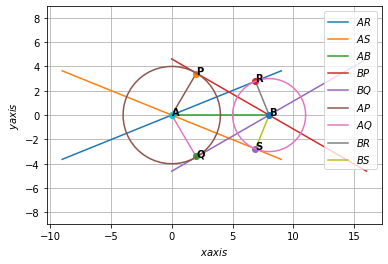
\includegraphics[width=\columnwidth]{Tangents on Circles with Centre A and B.png}
\caption{Tangents from centres of Circle}
\label{fig:circle}	
\end{figure}
\end{enumerate}
\end{document}